% !TEX encoding = UTF-8 Unicode

\documentclass[a4paper]{article}

\usepackage{color}
\usepackage{url}
\usepackage[T2A]{fontenc} % enable Cyrillic fonts
\usepackage[utf8]{inputenc} % make weird characters work
\usepackage{graphicx}

\usepackage[english,serbian]{babel}
%\usepackage[english,serbianc]{babel} %ukljuciti babel sa ovim opcijama, umesto gornjim, ukoliko se koristi cirilica

\usepackage[unicode]{hyperref}
\hypersetup{colorlinks,citecolor=green,filecolor=green,linkcolor=blue,urlcolor=blue}

%\newtheorem{primer}{Пример}[section] %ćirilični primer
\newtheorem{primer}{Primer}[section]

\begin{document}

\title{Medijska pismenost\\ \small{Seminarski rad u okviru kursa\\Tehničko inaučno pisanje\\ Matematički fakultet}}

\author{Ljiljana Mihajlović, Danica Šimšić,\\ Ana Stevanović, Tijana Zečević\\ kontakt email adresa autora}
\date{11.~novembar 2022.}
\maketitle


\abstract{
Motivacija za izradu seminarskog rada na ovu temu je činjenica da živimo u svetu informacija, i da je od opšteg značaja sposobnost prepoznavanja istinite, potpune i nepristrasne informacije, što medijska pismenost i jeste. Javnost je često nedovoljno informisana, a povremena predavanja stručnih lica u osnovnim školama na temu zaštite podataka na interentu i retke edukacije starijih generacija o ispravnom tumačenju medijskog sadržaja su površna rešenja. Iščitavanjem naučnih radova i sajtova za mlade došlo se do zaključka da je jedino rešenje ovog problema aktivno razvijanje medijske pismenosti. Za to je najpre potrebno razumeti način na koji mediji funkcionišu i razliku između tradicionalnih i društvenih medija, kao i pojmove spinovanja i dezinformacija, i kako ih prepoznati u stvarnom životu. 


Ključne reči : savremeni mediji, društveni mediji, medijska manipulacija, spinovanje, dezinformacije, kritičko mišljenje, medijska pismenost
}

\tableofcontents

\newpage

\section{Uvod}
\label{sec:uvod}

Razvoj tehnologije doveo je do intenzivnog prisustva medija u životu svakog pojedinca i jačanja medijskog uticaja na formiranje javnog mnjenja o društvenoj i političkoj stvarnosti. Gotovo neprimetno, mediji su iz sredstva informisanja prerasli u sredstvo informisanja i manipulacije. Mnoštvo informacija sa kojima smo svakodnevno u kontaktu, dobijeno iz različitih izvora i plasirano na različite načine, oblikuje javno mnjenje o društvenoj i političkoj stvarnosti.

Tokom sedamdesetih godina prepoznaje se potreba da se u obrazovne sisteme širom sveta uvede upoznavanje učenika sa osnovnim elementima i karakteristikama medija koji ih okružuju. 

Pojam medijske pismenosti uveden je 1992. godine na konferenciji o istoj (\emph{National Leadereship Conference on Media Literacy, 1992}), i definisan kao „sposobnost pristupa, analize, vrednovanja i slanja poruka posredstvom medija“ . Jednostavno rečeno, medijska pismenost je sposobnost da se objektivno, racionalno i kritičkim razmišljanjem prepozna \textbf{istinita}, \textbf{potpuna} i \textbf{nepristrasna informacija}.  
Stoga je najpre važno objasniti način funkcionisanja medija i značaj njihovog uticaja u savremenom društvu, da bi se razumela suština medijske pismenosti.

Neophodno je biti upoznat sa opasnostima i obmanama koje informacije tog tipa mogu doneti. Odnosno uvrstiti ispravnu analizu medijskog sadržaja u naše kritičko razmišljanje kako bismo znali proceniti šta je istina. Razvoj medija tokom decenija doveo je do potrebe za razvijanjem kako naše medijske pismenosti, tako i ostalih.

\newpage

\section{Medijska pismenost}

\subsection{Tradicionalni i društveni mediji}

	\textbf{{Mediji}} se definišu kao \emph{\textbf{{različiti kanali ili
			načini pomoću kojih se šire vesti, zabava,}}} \emph{\textbf{{marketinške
			poruke ili druge informacije.}}}

Skoro svi savremeni mediji su \textbf{masovni} mediji\footnote{Mediji čiji sadržaji dopiru do velikog broja ljudi}. Tome je doprinela
pojava interneta. Tako su se i tradicionalni mediji veoma brzo
„preselili`` na internet.
\bigskip

\begin{itemize}
	\item \textbf{Tradicionalnim medijima} smatra se bilo koji vid masovne
	komunikacije koji je postojao pre nego što je internet stupio na svetsku
	scenu. Tu se ubrajaju svi vidovi štampanih medija
	
	(slika\ref{fig:newspaper}), radio (slika\ref{fig:radio}), televizija (slika\ref{fig:tv}), pošta i poruke na
	javnim mestima.
\bigskip
	
	
\includegraphics[width=1.3in,height=1.225in]{slika 1.jpg}\label{fig:newspaper}
	
\includegraphics[width=1.3in,height=1.225in]{slika 2.jpg}\label{fig:radio}
	
\includegraphics[width=1.3in,height=1.225in]{slika 3.jpg}\label{fig:tv}
\bigskip

	Kod tradicionalnih medija komunikacija je \textbf{jednosmerna}, odnosno,
	kreatori medijskih poruka nemaju trenutnu povratnu informaciju o
	raspoloženju i reakciji koju je plasirana informacija izazvala. Važno je
	i ko je ciljana publika. Na primer, informacije o Met Gali\footnote{Met Gala je godišnji dobrotvorni događaj koji se organizuje svake godine u cilju prikupljanja novca za godišnju modnu izložbu koju organizuje modno odeljenje Met muzeja } je pogrešno plasirati putem radija, jer neće doći do ciljane publike.
\bigskip
	
	Treba imati u vidu da se tradicionalni mediji prilagođavaju životu u eri tehnologije. Skoro svaka tradicionalna medijska kompanija sada ima svoju veb stranicu ili aplikaciju, a često osnivaju i svoje zvanične profile na pojedinim društvenim mrežama, proširujući tako svoj uticaj i na njih.
\bigskip
	
	\item \textbf{Društveni mediji} su veb lokacije i aplikacije (slika\ref{fig:icons}). Za
	razliku od tradicionalnih medija, komunikacija je \textbf{dvosmerna}, a korisnici
	društvenih medija mogu sami da kreiraju medijske sadržaje i dele ih sa
	drugim korisnicima, kao i da jedni drugima šalju poruke kako bi
	diskutovali o problemima.
	
	\begin{figure}[h!]
	\begin{center}
		
\includegraphics[width=1.87842in,height=1.225in]{slika4.jpg}
	\end{center}
	\caption {Ikonice društvenih mreža}
	\label{fig:icons}
\end{figure}
	
	Osim mogućnosti kreiranja i objavljivanja sopstvenog medijskog sadržaja i dvosmerne komunikacije, kao bitna karakteristika društvenih medija izdvajaju se i društvene mreže, koje čine svi ljudi sa kojima komuniciramo preko interneta. 

\subsection{Spinovanje i manipulacija}
\label{sec:naslovN}

Za razvoj medijske pismenosti najpre se treba upitati ko proizvodi medijske poruke (država, pojedinac, izvesna medijska kuća…) i zašto ih proizvodi. Koji je cilj te medijske poruke? Kakva reakcija se očekuje i da li se određena informacija plasira u datom trenutku upravo zbog očekivane reakcije? 

U ovom poglavlju upoznajemo se sa terminom spinovanja.\textbf{Spinovanje} (eng. \emph{spin} - zaokret) je savremeni termin za vid medijske manipulacije koji obuhvata skup propagandnih trikova. Karakteristične metode spina podrazumevaju preuveličavanje izvesnih događaja i selektivno i tempirano iznošenje činjenica u javnost, najčešće u cilju preusmeravanja pažnje sa loših vesti i važnih problema na nevažne.

Činjenice iz nezvaničnih izvora se pojavljuju u medijima sa ciljem da izazovu burnu reakciju, zatim se poriču, pa opet tvrde, čime se manipuliše i novinarima. Sa sličnom namerom stvaraju se nepostojeći, često vrlo uznemirujući problemi kako bi se pored njih „provukli“ stvarni problemi, odnosno, kako bi ih javnost lakše prihvatila. 

Sposobnost razlikovanja činjenica od nečijeg mišljenja pomaže u razvijanju kritičkih i analitičkih sposobnosti, i svesti da nije sve uvek onako kao što izgleda. Dok se činjenicom smatra nešto što se može dokazati kao istinito, mišljenje se odnosi na lično uverenje i kako se neko oseća u vezi sa nečim. 

Većina metoda spina zasniva se na manipulaciji našim emocijama. Medijske poruke koje dolaze do nas imaju moć da nas navedu da osećamo tugu, uznemirenost, iznenađenje, ljutnju, radost, (nacionalni) ponos. Dr Den Sigel, naučnik u oblasti neurobiologije, razvio je princip „Prepoznaj i obuzdaj“ \cite {nameittotameit} (eng. \emph{Name it to Tame it}). Da bi se izbegla nagla reakcija i mogućnost da poverujemo u lažnu informaciju, važno je da zastanemo i pokušamo da definišemo emociju koju je medijska poruka izazvala. Gledano sa aspekta svrhe medijskog sadržaja, jedino je izveštavanje vid informisanja. Svi ostali sadržaji su vid ubeđivanja (tabela \ref{tab:tabela1}). 

Pošto je danas netačna informacija lako proverljiva, osmišljena je nova, mnogo podmuklija metoda manipulacije. Često se istovremeno plasiraju proverene informacije, poluistine i  dezinformacije, i na svima se insistira istim intenzitetom, na takav način da običan čovek počinje da veruje da su stvari ili mnogo bolje, ili mnogo gore nego što jesu, ali više nije siguran ni ko ga je u to ubedio, ni zašto u to veruje.

\begin{table}[h!]
\begin{center}
\begin{tabular}{|c|c|p{3cm} |} \hline
Vrsta sadržaja:& Vid:& Svrha:\\ \hline
Izveštavanje&Informisanja&Da definiše\\ \hline
Mišljenje &Ubeđivanja&Da utiče (na ono što verujete)\\ \hline
Oglašavanje &Ubeđivanja&Da utiče (na ono što kupujete)\\ \hline
Društveno oglašavanje &Ubeđivanja&Da utiče na to kako ćete da se ponašate\\ \hline
Pr &Ubeđivanja&Da utiče na to kako ćete da razmišljate o neko kompaniji\\ \hline
Propaganda &Ubeđivanja&Da utiče ili nametne neki politički sta, izbor itd.\\ \hline
\end{tabular}
\caption{ Svrha medijske poruke u odnosu na sadržaj.}
\label{tab:tabela1}
\end{center}
\end{table}

\newpage
\subsection{Dezinformacije}
\label{sec:naslovN}

Načini na koje se istina može izvrnuti su bezbrojni, s tim što treba podvući razliku između dezinformacija i lažnih vesti. \newline \textbf{Dezinformacije} u sebi sadrže delove istine, ili njeno pogrešno tumačenje, a za cilj imaju obmanjivanje javnosti. \newline \textbf{Lažne vesti} su jednostavno netačne informacije nastale usled greške ili lošeg novinarstva.    


U dezinformacije se ubrajaju parodija, podmetnuti, obmanjujući, fabrikovani i manipulisani sadržaj, lažna povezanost i lažni kontekst. U ovom poglavlju obradićemo samo neke od njih.


\begin{itemize}
    \item \textbf{Podmetnuti sadržaj} potiče sa sajtova čiji domen liči na domen zvaničnog sajta, tako da deluje kredibilno.
    \item \textbf{Obmanjujući sadržaj} predstavlja upotrebu informacija kako bi se stvorilo određeno javno mnjenje o nekoj ideji ili javnoj ličnosti, pri čemu može imati i pozitivan i negativan ton.
    \item \textbf{Fabrikovani sadržaj} je uvek lažan, a kreiran je isključivo radi obmane i nanošenja štete. Tu spadaju i dipfejk \cite{deepfake} (eng. \emph{deepfake}) video materijali.
    \item \textbf{Manipulisani sadržaj} predstavlja manipulisanje istinitim informacijama ili vizuelnim sadržajem u cilju obmane.
\end{itemize}


Pri prepoznavanju dezinformacija na internetu važno je obratiti pažnju na izvor (da li je legitiman) i internet adresu - treba biti oprezan sa domenima poput “.com.co”. Većina izvora sa reputacijom veoma vodi računa o gramatici i pravopisu, pa to može biti pokazatelj da je sadržaj fabrikovan. Obratiti pažnju na kredibilitet autora i obavezno proveriti tačnost informacija.


Najstariji i najrasprostranjeniji vid manipulacije u onlajn medijima upravo su 
senzacionalistički naslovi koji se popularno nazivaju \textbf{klikbejtovima} \cite{clickbait} (\emph{clickbait} – „mamac za klikove“). U ovakvim slučajevima, sadržaj članaka ili videoklipova ima malo do nikakve veze sa svojim naslovom. Cilj je privlačenje pažnje javnosti i reklamiranje oglasa. 


Deljenje dezinformacija ili lažnih vesti može da ima opasne i dalekosežne 
posledice. Obmanjujuće i netačne informacije često su tako „upakovane“ da se šire zapanjujućom brzinom, upravo zato što ljudi često ne razmisle pre nego što je podele. \newline
Ali bez obzira što su obmanjujuće i netačne, ove informacije takođe utiču na 
formiranje našeg mišljenja, na to kako glasamo, kako se lečimo, kako se hranimo… 



Zato je važno da \textbf{d o b r o} razmislimo pre nego što neku informaciju 
pošaljemo nekom ili je podelimo na svom profilu. 
U vreme izbijanja kovid pandemije UNESKO (eng. \emph{UNESCO}) je pokrenuo onlajn kampanju \newline
TakeCareBeforeYouShare \cite{unesco kampanja} (slika \ref{fig:takecarebeforeyoushare}), usled opasnosti koju dezinformacije i lažne vesti nose sa sobom. 

\begin{figure}[h!]
\begin{center}

\includegraphics[scale=0.4]{takecarebeforeyoushare.jpg}
\end{center}
\caption{Kampanja TakeCareBeforeYouShare}
\label{fig:takecarebeforeyoushare}
\end{figure}

\subsection{Medijska pismenost}
\label{sec:naslovN}

Tradicionalna definicija pismenosti odnosila se na sposobnost čitanja, pisanja i računanja. Danas ove tri sposobnosti podrazumevaju elementarnu pismenost. Pojam pismenosti u 21. veku je znatno proširen shodno zahtevima života u savremenom društvu.

Biti pismen znači biti u toku sa aktuelnim dešavanjima, biti komunikativan i razumeti probleme sveta koji nas okružuje. UNESKO je pismenost definisao kao:

\noindent \textit{"sposobnost identifikacije, razumevanja, interpretacije, komunikacije, računanja i kreiranja, korišćenjem pisanih, štampanih i vizuelnih materijala povezanih sa različitim kontekstima."}

Medijska pismenost definiše se kao sposobnost razumevanja, korišćenja i adekvatne interpretacije medijskih poruka, bilo da potiču iz društvenih ili tradicionalnih medija. Neophodno je posedovanje i drugih vrsta pismenosti kako bismo bili medijski pismeni, kao što su funkcionalna, društvena, kulturna, ekološka, digitalna, vizuelna, finansijska pismenost i druge (slika \ref{fig:literacies}).  

\begin{figure}[h!]
\begin{center}
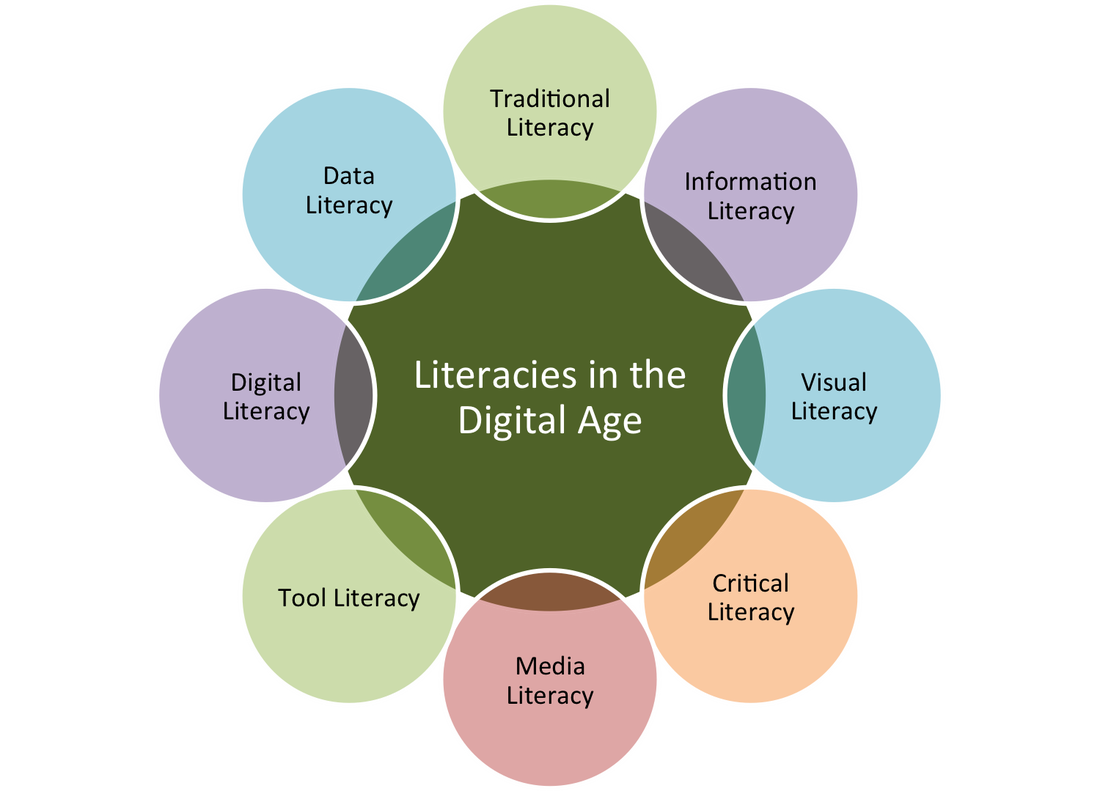
\includegraphics[scale=0.35]{literacies.png}
\end{center}
\caption{Vrste pismenosti u digitalnom dobu}
\label{fig:literacies}
\end{figure}

Medijska pismenost podrazumeva razumevanje kompleksnih medijskih poruka bilo kog oblika, njihovu grafičku analizu, zauzimanje stava povodom istih i preduzimanje koraka ka rešavanju problema ili promišljeno kreiranje novih poruka.

Analizu medijskog sadržaja možemo izvršiti pračenjem ovih koraka (tabela \ref{tab:tabela2}):

\begin{table}[h!]
\begin{center}
\begin{tabular}{|c|p{7cm}|p{5cm} |} \hline
Ključne reči:& Pet ključnih pitanja:& Pet suštinskhi koncepata:\\ \hline
Autorstvo&Ko je napisao poruku?&Sve medijske poruke su "konstruisane".\\ \hline
Format &Koje kreativne tehnike se koriste kako bi se privukla moja pažnja?&Medijske poruke su konstruisane upotrebom kreativnog jezika sa sopstevnim pravilima.\\ \hline
Publika &Kako različiti ljudi mogu ovu poruku razumeti drugačije od mene?&Različiti ljudi doživljavaju istu medijsku poruku na različit način.\\ \hline
Sadržaj &Koje vrednosti, životni stilovi i gledišta se prikazuju ili izostavljaju iz ove poruke?&Svaki medij ima ugrađene vrednosti i tačke gledišta.\\ \hline
Svrha &Zbog čega se ova poruka šalje?&Večina medijskih poruka je kreirana sa ciljem da ostvari profit i/ili moć.\\ \hline
\end{tabular}
\caption{ Ključna pitanja za analiziranje medijske poruke}
\label{tab:tabela2}
\end{center}
\end{table}

Ekspanzija medija dovela je do jačanja već moćnih korporacija i ekonomskih uticaja na plasiranje medijskih sadržaja, što navodi do zaključka da u savremenom dobu nismo mi više ti koji biraju informacije, već informacije biraju nas. Dolaze sa svih strana, a mi ih automatski usvajamo i ne razmišljamo o njihovom značenju i nameri onog ko ih šalje.

Vrlo je opasno što imamo uvid samo u jednu stranu priče, važno je imati i uvid u bar još nekoliko interpretacija medijskog sadržaja na određenu temu.

Medijska pismenost je delimično i nastala kao odgovor na komercijalizaciju kulture i "veliki prasak" informacija. Danas skoro svako naše saznanje potiče iz medija. Oni koji tvrde da mediji nemaju uticaj na njihov život treba da se zapitaju otkud im već izgrađeno mišljenje o ljudima koje nisu upoznali i aktuelnim dogadjajima kojima nisu prisustvovali.

Ranije je pristup informacijama bio ograničen, dok smo sada prezasićeni njima. Hteli mi to ili ne, mediji su sveprisutni deo naših života i bitno utiču na naše mišljenje. Ne treba da gradimo stav da "svi mediji lažu", ali je potrebno postaviti sebe u kritički odnos sa njima, što medijska pismenost i jeste.

\newpage
\section{Zaključak}
\label{sec:zakljucak}

Medijska pismenost je važna zato što nas uči da tumačimo različite vrste medija, interpretiramo i razumemo informacije i njihov izvor postavljajući prava pitanja, razlikujemo činjenice od mišljenja, promišljamo o medijskim porukama sa različitih tačaka gledišta i donosimo ispravne odluke. Pomaže nam da razlikujemo stvarnost od sveta koji su kreirali mediji. 


Važno je pomenuti da mediji bitno utiču na uspostavljanje društvenog sistema vrednosti. Medijska pismenost nas uči da razlučimo kojim medijima treba verovati, pa i tada uvek treba proveriti određenu informaciju, pre nego što je objavimo ili podelimo. Cilj je pronaći istinitu, nepristrasnu i potpunu informaciju u moru medijskog sadržaja.

\newpage

\addcontentsline{toc}{section}{Literatura}
\appendix

\iffalse
\bibliography{seminarski} 
\bibliographystyle{plain}
\fi

\begin{thebibliography}{9}


\bibitem{prirucnik1} Grupa autora (po azbučnom redu): Vlajković Bojić Violeta, Miladinović Nenad, Milijić Subić Dejana, Milošević Ivana. Priručnik za nastavnike \emph{ Naši učenici u svetu kritičkog mišljenja i medijske pismenosti}. Dostupno na adresi: https://zuov.gov.rs/prirucnik-za-nastavnike-nasi-ucenici-u-svetu-kritickog-misljenja-i-medijske-pismenosti/.

\bibitem{prirucnik2} Nedim Sejdinović i Tatjana Ljubić, \emph{Osnove medijske pismenosti – priručnik za učenike}, 2014. Dostupno na adresi:
http://www.medijskapismenost.net/dokument/Osnove-medijske-pismenosti---prirucnik-za-ucenike/.

\bibitem{preuzimanje1} Tabela \ref{tab:tabela1} preuzeta iz Priručnika za nastavnike \emph{ Naši učenici u svetu kritičkog mišljenja i medijske pismenosti}.

\bibitem{unesco kampanja} Dostupno na adresi: https://www.takecarebeforeyoushare.org/.

\bibitem{deepfake} Dostupno na adresi: https://www.youtube.com/watch?v=tRQWhOFFkBg.

\bibitem{clickbait} Dostupno na adresi: https://medijskapismenost.raskrinkavanje.ba/oblici-manipulacija-i-kome-se-obratiti-ako-ih-uocite/koji-sve-oblici-medijskih-manipulacija-postoje/klikbejt/.

\bibitem{nameittotameit} Dostupno na adresi: https://www.youtube.com/watch?v=ZcDLzppD4Jc.

\bibitem{newspaper} Dostupno na adresi: https://www.deutschland.de/en/topic/knowledge/national-newspapers

\bibitem{radio} Dostupno na adresi: https://economictimes.indiatimes.com/industry/media/entertainment/media/centre-asks-fm-radio-channels-to-refrain-from-using-vulgar-objectionable-content/articleshow/89919283.cms

\bibitem{tv} Dostupno na adresi: https://www.istockphoto.com/photo/an-old-tv-with-a-monochrome-gm1159377900-316990795

\bibitem{icons} Dostupno na adresi: https://www.motionvfx.com/store,mtracker-3d-social-media-icons-pack,p3588.html


\end{thebibliography}


\appendix


\end{document}

